\chapter{Problemanalyse}\label{ch:ch2label}
I dette kapitel analyseres forskellige problemstillinger, idrætsforeninger står overfor. I forbindelse med dette analyseres hvilke personer i foreningerne, der er relevante at interviewe i forbindelse med disse problemer. Den efterfølgende undersøgelse leder til en indskrænkning af et problem, som derefter bliver analyseret med det formål at ende med en problemformulering.
\par
Flere gruppemedlemmer i dette projekt har tidligere dyrket sport i en idrætsforening, hvilket har resulteret i en øget baggrundsviden. Grundet denne baggrundsviden er analysen rettet mod traditionelle idrætsforeninger fremfor foreninger, der tilbyder e-sport. Antallet af foreninger, der tilbyder e-sport, er også mindre end antallet af foreninger, der tilbyder mere traditionelle sportsgrene \citep{e-sport}. Derfor antages der at være rigere mulighed for at finde en traditionel forening med et problem.
\par
For at finde et problem i en idrætsforening er det fordelagtigt at vide, hvem der bliver påvirket af et eventuelt problem. Dette bliver i det følgende afsnit undersøgt i en interessentanalyse. 
\newpage
\section{Interessentanalyse}
Interessenterne er en stor del af projektet, da der skal laves et program specifikt for at løse deres problem. Denne undersøgelse vil blive brugt til at finde en retning for projektet og et mere afgrænset problem, som kan løses. Det er hermed relevant at forstå hvem interessenterne er, og hvad deres behov i forhold til problemet og dets løsning er. Derudover er det også vigtigt at forstå, hvilke krav de forskellige interessenter har til løsningen.

\subsection*{Forbund}
Et forbund er en samling af idrætsforeninger, som har lignende værdier og regelsæt. DGI og DIF er eksempler på forbund, der dækker over specialforbund, som arbejder med foreninger inden for en specifik sportsgren.
\par
Forbundet har ikke stor indflydelse på projektet, da der vil være mere fokus på de enkelte foreninger. Dog vil en løsning kunne påvirke forbundet gennem de enkelte foreninger, da det er nemmere at arbejde med velorganiserede foreninger. Derfor er det ikke relevant at kontakte et forbund, da der er fokus på de enkelte foreninger. 

\subsection*{Bestyrelse}
En af de større interessenter er bestyrelsen. Medlemmerne inden for bestyrelsen er som regel frivillige. Som bestyrelse har de stor indflydelse på projektet, da det er dem løsningen skal hjælpe, og de kommer til at blive direkte påvirket af projektet. Bestyrelsen har brug for en bedre og hurtigere måde at planlægge og organisere eksempelvis turneringerne, frivillige eller udstyr på. Ulempen ved dette kan være at, hvis ikke alle bruger systemet, kan der være sammenstød eller uoverensstemmelser med planlægningen. Det vil hermed være svært at holde styr på systemerne, hvis folk ikke bruger det samme program eller planlægningsmetode.
\par 
Gennem samtale med bestyrelsen kan mulige problemstillinger belyses. Der kan således uddrages konkrete problemer, som kan løses med et program. Bestyrelsen kan komme med forslag til potentielle egenskaber, der kunne være brugbare for dem. Dette vil ske gennem et semistruktureret interview, hvor interessenten får lov til at dele sine holdninger frit.

\subsection*{Frivillige}
De andre frivillige er også en vigtig interessent, fordi den anvendte planlægningsmetode i klubben har en væsentlig indflydelse på deres arbejdsopgaver. Da det er de frivillige, der ofte sidder med planlægningen, er det i deres interesse, at den anvendte metode optimeres. På den måde vil et program kunne formindske den tid, der bliver brugt på planlægningen. Deres behov kan hermed påvirke programmets udformning. Ulempen ved at introducere en ny metode er, at de frivillige skal lære at bruge programmet. Fordelen ved programmet vil være, at det bliver nemmere og mindre tidskrævende for den enkelte frivillige at planlægge eksempelvis turneringer, tidsplaner eller udskiftningen af slidt udstyr.\\
Det er hermed en mulighed at kontakte denne interessent, for at få afklaret hvilke behov der er i forhold til programmet.

\subsection*{Medlemmer}
Medlemmerne har en mindre rolle i forhold til, hvordan løsningen udvikles. De har ikke nogen indflydelse på programmet, da det ikke vil være dem, der bruger det. De kan dog blive påvirket af programmet, da optimering af klubbens ressourcer kan have en indflydelse på de aktiviteter, de deltager i. Hvis programmet ikke bliver brugt ordentligt, eller ikke er effektivt nok, vil det kunne få negative konsekvenser for medlemmerne, da der også er tale om potentiel spild af deres tid. Medlemmernes holdninger og ønsker i forhold til løsningen af problemet vil ikke blive taget i betragtning, da det er de frivillige og bestyrelsen, som kommer til at bruge programmet, og ikke medlemmerne.

\subsection*{Forældre}
Forældre til børn der er medlemmer af foreningen, er interessenter med en minimal indflydelse på programmets udvikling. De kommer ikke til at bruge programmet, de vil dog kunne mærke programmets virkning, især hvis der tidligere er sket fejl i planlægningen, og det så går ud over forældrenes tid og lyst til at deltage i aktiviteter. Eksempelvis kan der være problemer med organiseringen af faciliteterne, hvilket kan føre til dobbeltbookning af hallerne. Hvis forældrene i en sådan situation har kørt børnene til aktiviteten, er det spild af både forældrenes og deres børns tid. Sådanne tilfælde kan undgås, hvis man har et fungerende og effektivt program, der kan holde styr på disse ting.

\subsection*{Opsamling}
På baggrund af interessentanalysen udledes det, at der er forskellige interessenter, som bliver påvirket af en mulig løsning. For at få informationer om hvilke problemer en forening kan have, og som kan løses med et program, bliver der afholdt interviews med bestyrelsen. \\
Det er også valgt, at der interviewes forskellige slags foreninger. Dette gøres med det formål at finde enten et unikt problem, eller et bredere problem som flere forskellige foreninger har.\\

\section{Interviews}\label{Interviews}
I forbindelse med dette projekt er repræsentanter fra fire idrætsforeninger i Aalborg Kommune blevet interviewet. 
\par
Jonas Nielsen er et af bestyrelsesmedlemmerne for Aalborg Flyers FC. Foreningen blev stiftet i 1989 som den første floorball-klub i Danmark. Både børn, unge og voksne spiller floorball i foreningen \citep{AalborgFlyers}.
\par
Lars Segerstrøm er formand for Farstrup Boldklub, hvor der tilbydes både håndbold, fodbold, badminton og gymnastik. Foreningen har 350 ungdomsmedlemmer og 100 seniormedlemmer \citep{Farstrup}.
\par
Ina Breum er formand for AKG Gynmastik i Aalborg. Foreningen er stiftet i 1922 og har i dag 350 medlemmer. De tilbyder forskellige former for gymnastik for både børn og voksne, bl.a. springgymnastik og forældre/barngynmastik, samt yoga mm. for de voksne \citep{AKG}.
\par
Mogens Juul Møller er formand for Aalborg Karate Skole. Her undervises omkring 150 medlemmer i karate (Bilag \ref{ch:appElabel}).
\\\\
Gennem interviewene har tre emner vist sig at være potentielt interessante. Nedenfor gennemgås resultaterne af interviewene inddelt i disse emner. For referencer til interviewene henvises der til bilag \ref{ch:appBlabel}-\ref{ch:appElabel}, som er transskriptioner af hele eller udvalgte dele af hvert interview.

\subsection*{Udstyr}
Under interviewet med Jonas Nielsen fra Aalborg Flyers fortalte han, at der ikke var én specifik person, der var ansvarlig for deres udstyr. I stedet har frivillige et fælles ansvar for at holde øje med udstyret, i forbindelse med hvornår det er slidt og skal udskiftes. Der er ikke noget system, for hvordan dette gøres, men Nielsen viste ikke store bekymringer for, at det var et problem.
\par
I Farstrup Boldklub deles foreningen og den lokale skole om udstyret, mens klubben har ansvaret for at købe nyt ind. De har en ansvarlig for trøjerne til håndbold, da der ofte kommer harpiks på dem, så de bliver ødelagt og skal skiftes ud.
\par
AKG har deres eget udstyr, som de deler med Vester Mariendal Skole. De har dog noget særligt udstyr, som de gerne vil holde under opsyn. Ligesom hos Aalborg Flyers er der heller ikke her én bestemt person, som holder styr på udstyret. Alle kan kontakte bestyrelsen, hvis der er noget, der mangler, skal repareres eller udskiftes. 
\par
Det meste af Aalborg karateskoles udstyr er noget, medlemmerne selv ejer. De få redskaber, som foreningen selv har, er bl.a. måtter, sparkepuder og ekstra beskyttelsesudstyr. Da omfanget af udstyret er småt, og vedligeholdelsen er minimal, mener foreningens formand, Mogens Juul Møller, ikke, at det har været nødvendigt at have et system til at holde styr på disse.
\\\\
Generelt for de interviewede foreninger gælder det, at der ikke er et særligt system bag organiseringen af udstyr, men de har heller ikke problemer med det. 

\subsection*{Frivillige}
Aalborg Flyers har omkring 20 frivillige, hvor nogle få af dem påtager sig et større ansvar. Nogle frivillige fungerer som trænere, mens eksempelvis forældre nogle gange hjælper til ved arrangementer. Under turneringer skal der laves en dommerplan over hvilke frivillige, der fungerer som dommer til hver kamp. Dommerplanen lægges manuelt, og der forsøges at finde optimale tider, for hvornår kampene skal spilles. Der opleves også problemer med manglen på medlemmer, der aktivt melder sig som dommere. Dette løser de ved at lave faste planer, og derefter er der mulighed for internt at bytte tider.
\par
I forbindelse med organisering af frivillige i Farstrup Boldklub nævner Lars Segerstrøm, at opgaver bliver uddelegeret gennem mundtlige aftaler. Når der eksempelvis i slutningen af en sæson skal udnævnes trænere, sker det, ved at de nuværende trænere får muligheden for enten at fortsætte eller tage en pause. Hvis der derefter er nogle poster, der mangler at blive dækket, går bestyrelsen i gang med at spørge, om der er nogle andre fra lokalsamfundet, der har lyst.
\par
Ina Breum fra AKG gymnastikforening fortæller, at kommunikationen mellem bestyrelsesmedlemmerne og de frivillige ofte sker gennem e-mail eller Facebook. Dog blev Facebook mest brugt til hurtige spørgsmål, da det ikke er alle, der har en bruger. På den måde undgår de, at der er nogen, som ikke får de vigtige informationer at vide. Derudover er der et bestyrelsesmøde hver anden måned, hvor forskellige emner og foreslag bliver bragt på banen.
\par % [11:55]
Aalborg karateskoles frivillige består hovedsageligt af bestyrelsesmedlemmer og instruktører. Måden hvorpå de frivillige bliver organiseret, er gennem instruktørmøder, hvor der aftales, hvem der tager hvilke hold og hvornår. Der er senere mulighed for at bytte tider internt mellem instruktørerne. Derudover kommunikeres der gennem e-mails. De har hermed ingen systemer til at holde styr på organiseringen af deres frivillige, da det ikke menes at være nødvendigt.
\\\\
Foreningerne har hver deres metoder til at organisere deres frivillige på. Alle foreningerne har hver især fundet den bedste måde at kommunikere internt, eksempelvis gennem mund til mund aftaler, mail eller Facebook. Der blev ikke fundet større problemstillinger under interviewene i forhold til organisering af frivillige.
% Dette kan være et problem, hvis nu man er en del af flere ting - Liv 09/11-2018 (LIVS FØDSELSDAG)

\subsection*{Turneringer}
Jonas Nielsen fra Aalborg Flyers gav udtryk for udfordringer med planlægningen af turneringer. Den metode der bliver benyttet nu, er ved at bruge Excel som værktøj. Nielsen fortæller at problemerne opstår, når der skal laves ændringer i den færdige plan. Et eksempel kunne være, at hvis et hold melder afbud, kan det være nødvendigt at lave det hele om, da planen ikke længere vil give mening. Dette resulterer i meget spildt arbejde og tid. Nielsen fortæller ligeledes, at han tidligere har oplevet store fejl i planlægningen af turneringer (Bilag \ref{ch:appClabel}). Dette kunne have været undgået, hvis planlæggerne i stedet havde brugt et program til at lægge planen.
\par
Farstrup Boldklub holder også turneringer, hvor udvalgene for de forskellige sportsgrene står for planlægningen. Der bliver eksempelvis arrangeret stævnedage, hvor der er flere hold, som spiller i løbet af dagen. Ligesom i Aalborg Flyers bruger Farstrup Boldklub også Excel som værktøj. Det er dog ikke et fast værktøj, da der også planlægges ved nedskrivning i hånden.
\par
AKG gymnastik deltager ikke i turneringer. De laver dog opvisninger, hvor det kun er foreningens egne medlemmer, der deltager. For disse opvisninger bliver der ikke brugt noget decideret planlægningsværktøj, da de kun skal organisere deres eget hold. % [14:05]
\par
Aalborg karateskole deltager både i store og små turneringer. De store turneringer bliver planlagt et stykke tid før, hvor de mindre turneringer fastsættes dagen forinden. Planlægningen af turneringsplanerne sker igen i Excel. 
\\\\
Den måde hvorpå der planlægges, sker generelt manuelt, hvor der enten bruges Excel eller også foregår det i hånden på papir. Dette kunne optimeres gennem et system, der også vil gøre det nemmere at foretage ændringer i kampprogrammer, uden større vanskeligheder.

\subsection*{Opsamling}
På baggrund af interviewene er der blevet fundet problemstillinger i emnerne udstyr, frivillige og turneringer. Problemerne om udstyr fravælges, fordi problemer med slidt udstyr er trivielt, og kræver ikke mange kræfter at holde under opsyn.
\par
På samme måde fravælges organiseringen af frivillige, da der her ikke var en konkret eller stor nok problemstilling at arbejde videre med.
\par
Turneringer er således blevet valgt. Dette er gjort, fordi turneringsplanlægning er et konkret problem, som kunne blive forbedret ved hjælp af et program. Samtidig er turneringsplanlægningen et specifik og afgrænset område, som ikke er et trivielt problem, hvis der hele tiden skal ændres i planen.

\section{Turneringer}
Der findes rigtige mange forskellige former for turneringer. De har næsten alle det samme formål - at finde den bedste i sportsgrenen - men de bliver afviklet på forskellige måder. Et eksempel kunne være kata i karate, hvor man kan dyste om hvem der er bedst til at lave øvelser af varierende sværhedsgrad (Bilag \ref{ch:appElabel}). Samtidig spiller man i fodbold mod hinanden for også at finde det bedste hold, men det er mere direkte end kata. Turneringerne i de forskellige sportsgrene går stort set ud på det samme, men der er små forskelle mellem dem, og regler for op- og nedrykning kan variere. Baseret på dette og resultatet af interviewene er det derfor blevet valgt at fokusere på floorballs regler for turneringer i denne rapport.

\subsubsection{Landsturneringer}
Danmarksturneringen i floorball er en landsdækkende turnering, der løber gennem en hel sæson. Den begynder i september og slutter i april \cite{Landsturnering}. Turneringen er delt op i to regioner – vest og øst. De øverste divisioner har op- og nedrykningskampe, mens de nederste divisioner bliver rykket op og ned baseret på point i slutningen af sæsonen.
\par
Kampe afvikles ved brug af et cup-system (Figur \ref{fig:cup-spil}). Der er først et grundspil, hvor alle hold bliver opdelt i et antal af puljer, og så bliver der spillet indbyrdes. Derefter skal de bedst placerede i hver pulje dyste mod hinanden. Vinderne går videre til næste runde, og sådan forløber resten af turneringen, indtil der er to finalister tilbage. I figuren er der et eksempel på dette system med 10 hold i én region \cite{Unihoc}\cite{Landsturnering}.

% Billede
\begin{figure}[H]
  \centering
  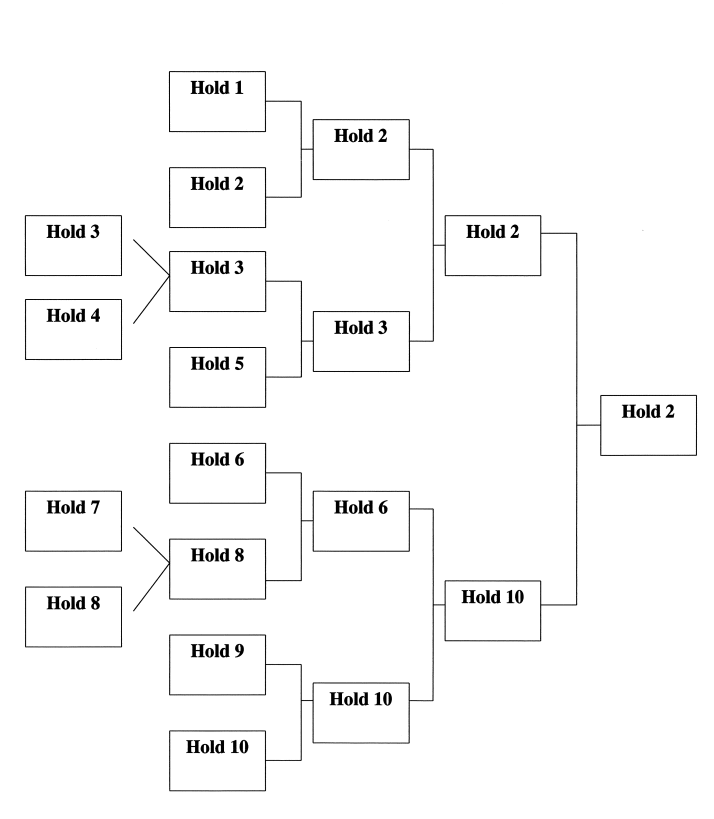
\includegraphics[width=0.7\textwidth]{figures/cup-spil.png}
  \caption{Cup-system med 10 hold 
  \citep{staevnemappe}. }
  \label{fig:cup-spil}
\end{figure}

Sidst på sæsonen vil der være en finale for at afgøre vinderen af de to resterende hold. Landsturneringen varer en hel sæson, så der er meget, der skal laves, både før og imens sæsonen er i gang. Jonas Nielsen fra Aalborg Flyers siger, at deres bestyrelse bruger meget tid på at få planlægningen til at fungere. Det er ikke kun forbundet, der arbejder med turneringen - idrætsforeningerne er meget involveret i planlægningen gennem hele sæsonen (Bilag \ref{ch:appClabel}). % (citat: linje 148 i bilag C) 

\subsubsection{Pokalturneringer}
I modsætning til landsturneringerne er alle regler om divisioner og deres niveau ophævet i pokalturneringen. Dette gør turneringen tilgængelig for alle hold, uanset hvilken division de er i. Pokalturneringen gør også brug af cup-systemet, men den afvikles hurtigere, da den ikke varer hele sæsonen. Turneringen begynder i august og er færdigafviklet i januar måned \cite{Pokalturnering}. Den har meget tilfælles med landsturneringen, men den er kortere, så den tager tid at planlægge, men ikke lige så meget som landsturneringen gør.

\subsubsection{Stævner}\label{staevner}
Stævnerne er mere hyppige end de andre turneringer og bliver afviklet på én dag i løbet af weekenden. Selvom ældre også kan deltage i stævner, er det som oftest ungdommen, som deltager regelmæssigt hos Aalborg Flyers (Bilag \ref{ch:appClabel}).
\par
Stævnerne foregår hver måned, og idrætsforeningerne skiftes til at være vært (Bilag \ref{ch:appClabel}). De bestemmer selv hvordan deres eget stævne skal organiseres. Før sæsonen begynder, planlægger idrætsforeningerne og forbundet, hvornår alle hver især skal holde stævne. Dette giver bestyrelserne god tid til at planlægge og organisere faciliteter til stævnerne. 
\\
% Billede
\begin{figure}[H]
  \centering
  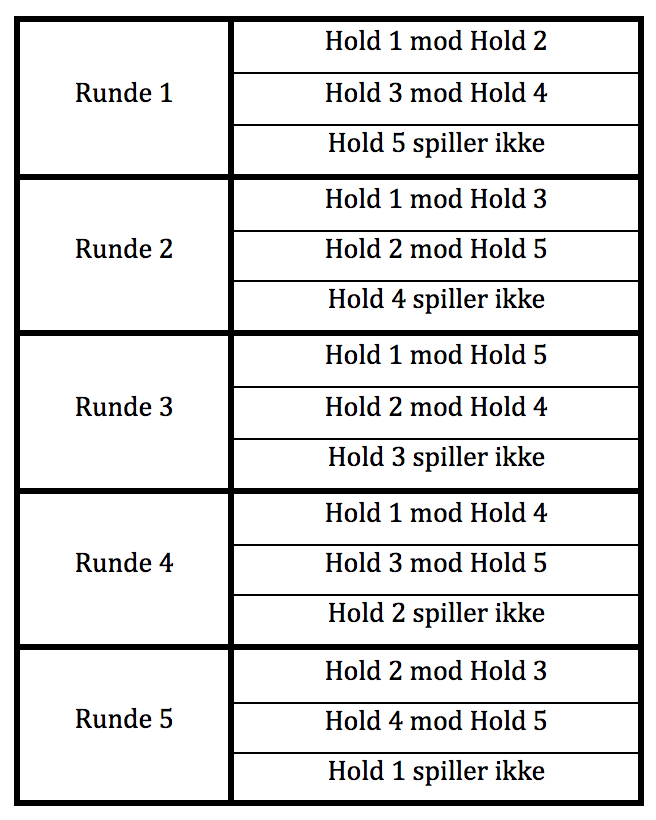
\includegraphics[width=0.6\textwidth]{figures/RoundRobin.png}
  \caption{Turneringssystem, hvor alle spiller mod alle. Eksemplet er med 5 hold over 5 runder}
  \label{fig:RoundRobin}
\end{figure}

Der er flere måder at afvikle stævnerne på. Ældre årgange bruger cup-systemet, og for børn bliver stævnet afviklet ved hjælp at et nyt koncept, som de seneste par år er blevet mere udbredt i Danmark. Det er et koncept, der bruges af flere sportsgrene, som er tilrettet til børn. Formålet er at få flere børn til dyrke idræt og sætte fokus på sjov frem for konkurrence \citep{kidzRegler}.
\par
Floorball har lavet en KidzLiga, som følger dette fokus. I ligaen er der niveauinddeling på fire rækker, hvor børnene bliver sat på niveauer, som matcher deres sportskompetence. Dette er en ny måde at opdele spillere på i forhold til den traditionelle måde, hvor der blev opdelt efter alder.
\par
Turneringen er opdelt i fire regioner: Nord, Syd, Midt og Øst. Kampene bliver afviklet anderledes end i de andre turneringstyper. Reglerne siger, at hvert hold som udgangspunkt skal spille 6 kampe til et stævne, men der er ikke specifikke regler for hvor mange gange to hold må spille imod hinanden. Alle hold skal have en eller flere hvilekampe, dvs. at der skal ikke være hold, som spiller to gange i træk. Børnene spiller på mindre baner, og hver kamp bliver afviklet på 6 minutter. Der kan ikke optjenes point til stævnerne, hvilket gør, at der ikke er nogen vindere eller tabere i ligaen \citep{kidzRegler}.
\par
Alle disse kriterier gør, at det ikke er muligt at bruge cup-systemet til at afvikle kampe på. KidzLigaen har et andet formål og et anderledes sæt af regler, som skal følges.

\subsubsection*{Opsamling}
De store lands- og pokalturneringer planlægges af forbundet. Da denne planlægning er ude af foreningernes hænder, fravælges det her at fokusere på dem. I stedet, vil der blive fokuseret på stævner, da disse bliver planlagt og organiseret af den lokale forening. Denne planlægning er ikke altid lige god (se afsnit \ref{Interviews}), og det vil derfor være et godt område at fokusere på i projektet.
\par
For at afgrænse projektet, vælges det at fokusere på KidzLiga, da der er blevet fundet konkrete eksempler på problemer i dette område (Bilag \ref{ch:appClabel}). 

\subsection{Planlægning af stævner}
I dette afsnit beskrives det hvordan et stævne i KidzLiga floorball arrangeres. Denne måde at planlægge og afvikle en tunering på kan gælde for andre sportsgrene, men dette afsnit omhandler specifikt KidzLiga floorball.
\par
Floorball Danmark er et specialforbund med det formål at give interesserede personer mulighed for at spille floorball. En forening, der ønsker at arrangere et KidzLiga-stævne, kan vælge at indsende en formular til Floorball Danmark, hvorefter de arrangerer det, eller foreningen kan arrangere stævnet på egen hånd. Stævnerne arrangeres lokalt eller regionalt, og forbundet forsøger at afholde mindst ét stævne i måneden i hver region \citep{kidzRegler}.
\par
Hvis Floorball Danmark arrangerer stævnet, tager de sig af promovering og tilmelding til stævnet. Derudover udarbejder de et kampprogram, der tilsendes værtsforeningen fem dage før stævnet. Foreningen har herefter mulighed for selv at redigere programmet, og har pligt til at rette det til, i tilfælde af afbud.
\par
Foreningen skal selv sørge for, at der er udstyr tilgængeligt, og at der bliver opstillet baner. Det er også værtsforeningen, der skal afvikle stævnet, ved eksempelvis at have dommere til kampene, og sørge for at der er tilstrækkeligt mandskab\citep{kidzRegler}. 
\par
Aalborg Flyers arrangerer selv deres stævner. De sender selv invitationer ud til andre floorball-foreninger, ofte via Facebook eller mail. De arrangerer også turneringer for skoler, bl.a. til Skolernes Floorball Dag. Ved planlægning af disse inddeler Aalborg Flyers de tilmeldte hold efter alder og evt. i puljer indenfor hver aldersrække hvis nødvendigt. Til opstilling af programmet bruges en skabelon i Excel. Dette kan være et stort arbejde, især hvis der senere skal laves ændringer i programmet.

\subsection*{Opsamling} 
En floorball-forening har forskellige muligheder for at planlægge stævner. Ligegyldigt om kampprogrammet for en turnering er planlagt af Floorball Danmark eller af den enkelte floorball-forening, kan det være tidskrævende og besværligt at skulle redigere det i tilfælde af afbud, især når de først får besked på dagen for turneringen.
\par
Som det også er beskrevet i afsnit \ref{Interviews}, kan der være problemer med at foretage ændringer i kampprogrammet. Derfor vælges det at arbejde videre med problemet angående fleksibilitet af turneringsplanlægning.

\section{Analyse af eksisterende programmer}
Der findes forskellige programmer til forskellige turneringssystemer. Af de interviewede idrætsforeninger bruger ingen disse programmer. De bruger i stedet Excel eller lignende til organisering af turneringer. Excel kan være et godt og detaljeret værktøj, men kan være svært at bruge. Derfor kan det være en fordel med et dedikeret program til turneringsplanlægning, som er mere simpelt at bruge.\\
For at sikre at der ikke findes eksisterende eller lignende værktøjer, der løser problemstillingen, laves denne konkurrentanalyse.
\par
Tournament Scheduler og Teamopolis er eksempler på hjemmesider, der producerer kampplaner for turneringer, hvor alle spiller mod alle. Man indtaster forskellige oplysninger som holdnavne, lokation, og om holdene skal spille mod hinanden en eller to gange. Derefter får man en liste over hvilke holde, der spiller mod hinanden i hver runde. I tilfælde af Tournament Scheduler er der mulighed for at redigere i listen for at ændre holdnavne, samt tilføje point og eventuelle noter. Hjemmesiden generer også en rankingside, hvor man kan få et overblik over hvilke hold, der eksempelvis har vundet eller tabt flest runder. Derudover udregnes, hvor mange gange hvert hold har spillet på det nuværende tidspunkt i turneringen.
\par
Begge hjemmesider har dog visse begrænsninger. Der er kun muligt at lave en turneringsplan, hvor alle hold spiller mod hinanden. Dette kan være en ulempe, hvis der er mange hold, som skal spille mod alle, da det kan tage for lang tid at komme i gennem alle kampene. De giver desuden ikke mulighed for at blande holdene, i tilfældet at man ønsker en anden holdopsætning. Brugeren er selv nødt til at ændre på rækkefølgen af holdnavnene \citep{Teamopolis}\citep{TournamentScheduler}.
\\\\
Disse hjemmesider er ikke optimale til at planlægge KidzLiga turneringer, da der ikke tages højde for de regler, der er stillet i turneringen (Se afsnit \ref{staevner}). Derfor er det stadig et problem, der skal løses. 